The transfer function between drive force $F(s)$ and velocity $V(s)$ for a car is given by 

\[
\frac{V(s)}{F(s)} = G(s) = \frac{1}{1000s+100}
\]

\begin{flushleft}
The car is controlled by the PI controller
\end{flushleft}

\[
C(s) = \frac{K_p s+K_I}{s}
\]

\begin{flushleft}
and the controller and plant are placed in the standard negative unity feedback configuration shown in the figure below. The settling time in response to a unit step reference input must be less than 4.6 seconds.
\end{flushleft}

\begin{center}
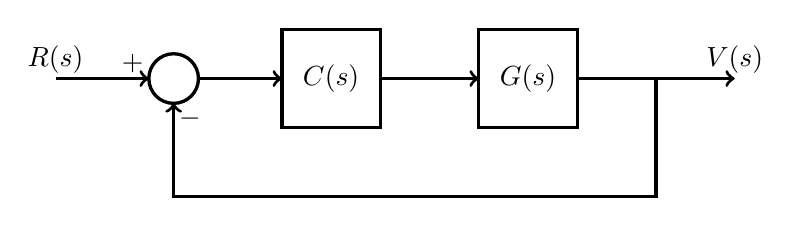
\begin{tikzpicture}[scale=1,inner sep=0pt,outer sep=0pt,very thick,
sysblock/.style={draw,rectangle,inner sep=2pt,minimum width=1.25cm,minimum height=1.25cm,inner sep=4pt, very thick}]
\draw (1.5,0) node[draw,circle] (sum1) {$\rule{0pt}{18pt}$};
\draw (3.5,0) node[sysblock] (K) {$C(s)$};
\draw (6,0) node[sysblock] (G) {$G(s)$};
\draw[->] (0,0) node[above=2pt] {$R(s)$} -- (sum1.180) node[above left=2pt] {$+$};
\draw[->] (sum1.0) -- (K.180);
\draw[->] (K.0) -- (G.180);
\draw[->] (G.0) -- ++(2,0) node[above=2pt] {$V(s)$};
\draw[->] (G.0) ++(1,0) -- ++(0,-1.5) -| (sum1.-90) node[below right=2pt] {$-$};
\end{tikzpicture}
\end{center}

\begin{flushleft}
Find all necessary constraints on the parameters $K_p$ and $K_I$ such that the closed-loop step response meets the settling time requirement. \textit{Note: although the solutions use the Routh Hurwitz test from prior semesters, recall that a sufficient condition for second-order systems to be BIBO stable is for all of the coefficients on $s^2$, $s^1$, and $s^0$ in the denominator be greater than zero. This condition does not apply to higher-order conditions.}
\end{flushleft}
